
\textbf{Магнитное поле}. Для использующегося зеемановского замедлителя зависимость \cite{vlad} магнитного поля $\sub{B}{exp}$ от координаты $z$ представлена на рис. \ref{fig:zB}. В соответсвие с \cite{stack} магнитное поле эффективно замедляет атомы, при  $B(z) \propto \sqrt{1-z/z_0}$, на рисунке \ref{fig:zB} видно, что эта зависимость достаточно хорошо приближает $\sub{B}{exp}(z)$.
Параметры аппроксимации: $z_0 = \meas{94}{1}{см}$, $\delta z = \meas{15}{1}{см}$, $B_0 = \meas{740}{13}{Гс}$, $B_1 = \meas{260}{12}{см}$. 

\begin{figure}[h]
    \centering
    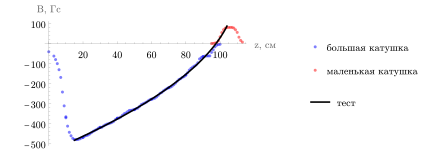
\includegraphics{figs/Bz.pdf}
    \caption{Зависимость магнитного поля внутри зеемановского замедлителя от координаты}
    \label{fig:zB}
\end{figure}

\textbf{Тормозящая сила}. 
Считая, что мы работаем с циклическим переходом \red{(указать каким)}, в приближение двухуровневой системы, эффективное сила, действующая со стороны лазерного луча на атом, может быть записана в виде\footnote{
    Нагрев, связанный с изотропным излучением фотона, приводящий во время движения к случайным блужданиям в пространстве поперечных скоростей в данной работе не рассматривается, потери связанные с этим эффектом обычно ограничиваются 10\% \red{(добавить ссылку)}. 
}  \red{(добавить ссылку)}
\begin{equation*}
    F = \frac{\hbar k \Gamma}{2} \frac{s}{1+s+4({\delta}+k v)^2/\Gamma^2}
\end{equation*}
где $s=I/\sub{I}{sat}$ -- параметр насыщения, $\sub{I}{sat}$ -- интенсивность насыщения, $v$ -- скорость атома, $k$ -- волновой вектор. 

Уравнение движения запишется в виде
\begin{equation*}
    \frac{d v}{d t} = \frac{F}{m},
    \hspace{0.25cm} \overset{v \d t = \d z}{\Leftrightarrow}  \hspace{0.25cm}
    \frac{d v(z)}{d z} = \frac{F(v, z)}{m \, v(z)},
\end{equation*}
где $m$ -- масса атома. Таким образом можем найти зависимость $v(z)$ для различных $v_0 \overset{\mathrm{def}}{=} v(z=0)$, характерный вид приведен на рис. \ref{fig:vZz} для $\delta = -20\Gamma$, $s=20$, $B(z) \approx \sub{B}{exp}(z)$.
\begin{figure}[h]
    \centering
    \subfigure[]{\includegraphics{figs/vz.pdf}}
    \hspace{10 mm} 
    \subfigure[]{\includegraphics{figs/vdist_v2.pdf}}
    \vspace{-3mm}
    % zeeman_sim_v2
    \caption{a) Зависимость скорости атомов от координаты в зеемановском замедлителе. b) Характерное преобразование распределения атомов по скоростям после замедления}
    \label{fig:vZz}
\end{figure}

% заменить график на отнсительные величины

Для атомов со скоростями $v < \sub{v}{crit}$ замедлитель работает эффективно и замедляет до некоторой характерной $\sub{v}{slow}$, рядом с которой атомы распределены на масштабе \red{(добавить ссылку)} $\frac{1}{2}\Gamma\sqrt{1+s} / k$, характерное преобразование распределения\footnote{
    \textit{Забавный факт}. Впервые данный способ охлаждения атомов применялся \cite{__1981} для охлаждения Na до 1.5\,К в продольном направление  в 1981 году.
}  атомов по скоростям приведено на рис. \ref{fig:vZz}b, полученное в результате моделирования методом Монте-Карло для $10^5$ частиц. Обычно для зеемановского замедлителя выполняется, что $\sub{v}{crit} < \alpha$. 


% ~ 2 м/c * sqrt(1+s)


\newpage
\textbf{Эффективность замедлителя}. Рассмотрим поток частиц, долетающих до замедлителя с учётом геометрии системы: $v_r/v_z < \sub{\varphi}{in} \sim 1/40$. Частицы распределены в соотвествии с \red{(добавить ссылку)}
\begin{equation}
    f(v_z, v_r) \propto v_r e^{-(v_r/\alpha)^2} v_z e^{-(v_z/\alpha)^2} \theta(\sub{\varphi}{in} - v_r/v_z).
    \label{ftheta}
\end{equation}
В дальнейшем в моделировании будет использоваться $10^6$ частиц из распределения \eqref{ftheta} для $\alpha = 300\un{м/c}$.

\begin{figure}[h]
    \centering
    \rotatebox{90}{\hspace{12mm}\scalebox{0.8}{$B_0=500\un{Гс}$}}
    \hspace{2 mm} 
    \includegraphics{figs/etas_v2.pdf}

    \rotatebox{90}{\hspace{12mm}\scalebox{0.8}{$B_0=700\un{Гс}$}}
    \hspace{2 mm} 
    \includegraphics{figs/etas_v1.pdf}
    \caption{Эффективность работы замедлителя}
    \label{fig:eta}
\end{figure}

Lorem ipsum dolor sit amet, consectetur adipisicing elit, sed do eiusmod
tempor incididunt ut labore et dolore magna aliqua. Ut enim ad minim veniam,
quis nostrud exercitation ullamco laboris nisi ut aliquip ex ea commodo
consequat. Duis aute irure dolor in reprehenderit in voluptate velit esse
cillum dolore eu fugiat nulla pariatur. Excepteur sint occaecat cupidatat non
proident, sunt in culpa qui officia deserunt mollit anim id est laborum.

\begin{figure}[h]
    \centering
    \rotatebox{90}{\hspace{12mm}\scalebox{0.8}{$B_0=700\un{Гс}$ \hspace{29 mm} $B_0=500\un{Гс}$}}
    \hspace{2 mm} 
    \includegraphics{figs/etas_v3.pdf}
    \caption{Эффективность работы замедлителя}
    \label{fig:eta2}
\end{figure}


Lorem ipsum dolor sit amet, consectetur adipisicing elit, sed do eiusmod
tempor incididunt ut labore et dolore magna aliqua. Ut enim ad minim veniam,
quis nostrud exercitation ullamco laboris nisi ut aliquip ex ea commodo
consequat. Duis aute irure dolor in reprehenderit in voluptate velit esse
cillum dolore eu fugiat nulla pariatur. Excepteur sint occaecat cupidatat non
proident, sunt in culpa qui officia deserunt mollit anim id est laborum.

